\section[head={SC2}, tocentry={StarCraft II}, reference={SC2}]{StarCraft II} \label{sec:sc2}
StarCraft II (SC2) is a real-time strategy (RTS) online video game created by Blizzard Entertainment. It is a popular multiplayer game with three million copies sold worldwide within its first month of sale, after its release in July 2010 \cite{blizzard2010sales}. In terms of competitions, several tournaments are held so players around the globe can compete against each other. The biggest tournament, the \textit{World Championship Series Global Finals}, is organized by the game publisher. In order to qualify for the finals, players from various regions are competing in series of events, the \textit{StarCraft II World Championship Series}. In the finals, all matches are one versus ones (1v1), leading to 16 participants competing against each other on a stage in South Korea and continued in North America. These series exist since 2016 and the prize pool of \$2 million is always spread among the events in the series \cite{MajorTou70:online}.

\subsection{Gameplay}
In SC2 players are competing against each other on a grid-like map, which is visible as a miniature version on the bottom left part of the screen and referred as \textit{minimap}. The information players can access is limited by \textit{Fog of War}, as seen in figure \ref{fig:sc2_minimap}. Fog of war is a feature that limits the players' information to only areas on the map, which are revealed by allied units. On the minimap, as well as the normal map, this information is indicated by dark areas for unrevealed and light areas for revealed \cite{liquipedia_fog}. 
\begin{figure}[H]%
\centering
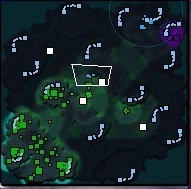
\includegraphics[width=4cm, height=4cm]{source/images/sc2_minimap}%
\caption[Minimap in SC2]{Minimap in SC2. The green elements belong to player 1 and the purple ones to player 2, while the white elements are neutral. The terrain of the map, as well as the neutral units, are visible but not necessarily revealed, due to absence of allied units (indicated by green elements). Source: Adapted from \protect\cite{Starcraf92:online}}%
\label{fig:sc2_minimap}%
\end{figure}
There are different ways to play the game, but in esports the most competitive one is the 1v1 game mode. Players have to choose among three races: Terran, Zerg and Protoss. Each race has different advantages and disadvantages; therefore, players have to adapt strategies and play-styles accordingly. Every player starts with one Townhall and 12 worker units, who are responsible for collecting resources and store them in the Townhall. Resources are used to buy buildings, which enable the production of more units and the unlocking of new technologies. Units serve the purpose of attacking the enemy, or collecting resources (workers). The management of these concepts are termed as macro and micro. Macro refers to the management of players economy and technology, i.e., gathering resources, spending them on new buildings and upgrading to newer technologies, while micro refers to the management of players' army, i.e., moving, attacking, retreating if necessary \cite{liquipedia_sc2}. To win a game, a player has to balance micro and macro management, while performing following tasks:
\begin{enumerate} 
	\item collect resources (minerals and vespene gas)
	\item construct buildings
	\item amass an army
	\item destroy all enemy buildings \cite{2017arXiv170804782V}
\end{enumerate}

The performance of players skill level is based on points, which are earned, or lost by winning or losing matches. To measure that, the MMR (Matchmaking Rating) is used, which aims to rank players in a way, that they have a 50\%-win ratio against other players with similar skill level. Based on the MMR, players are ranked from the lowest to highest league: Bronze, Silver, Gold, Platinum, Diamond, Master and Grandmaster \cite{liquipedia_mmr}. 
\begin{figure}[h]
 \centering
 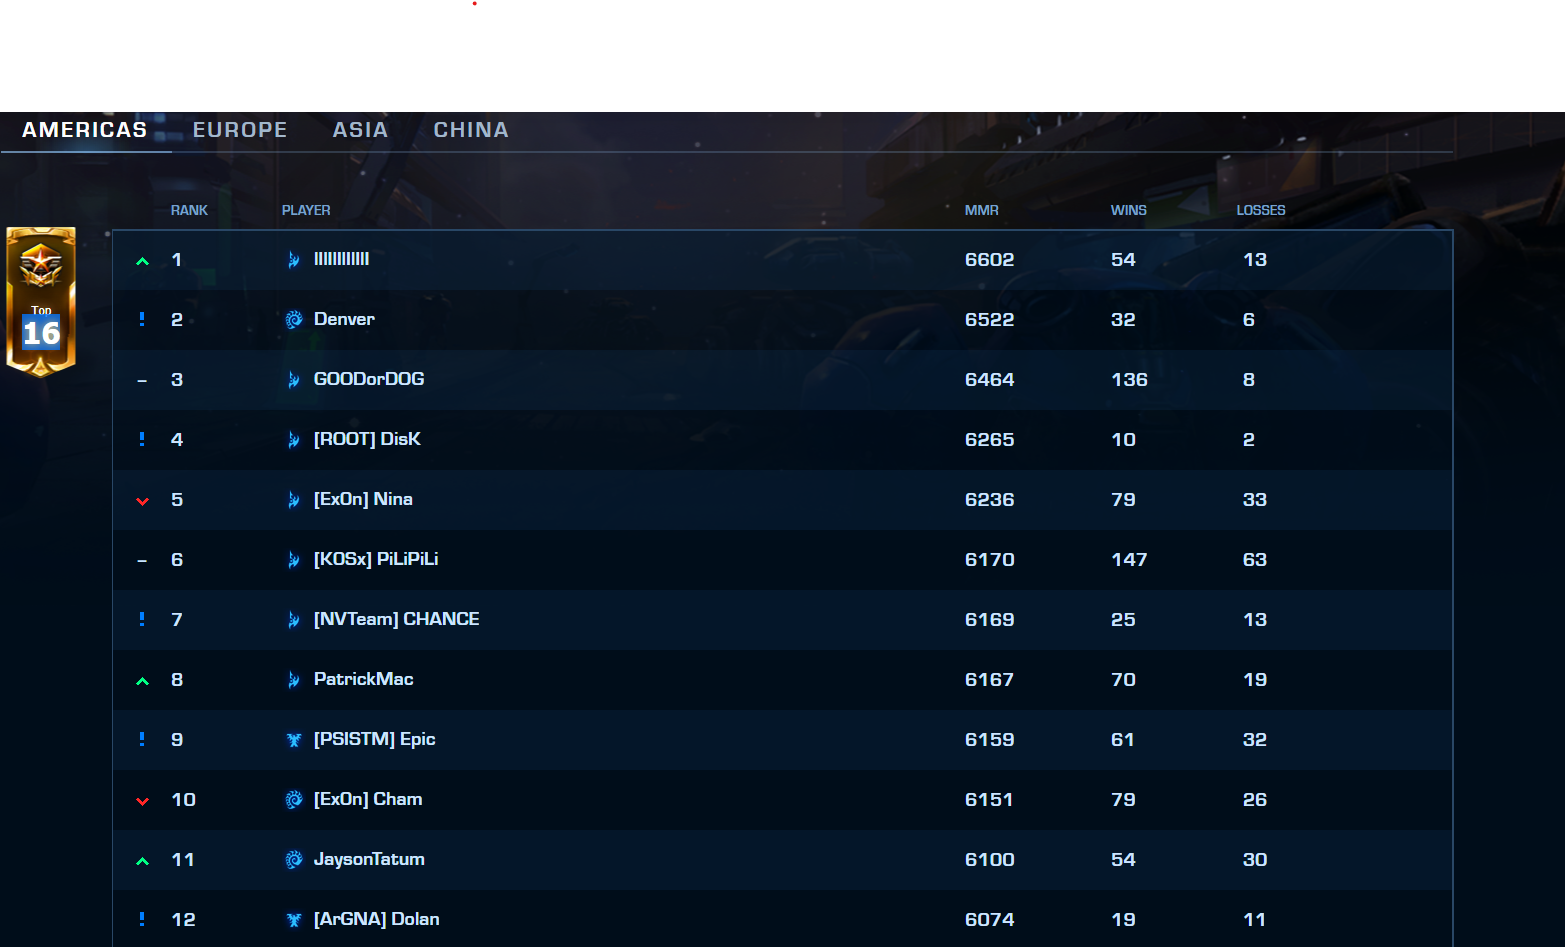
\includegraphics[height=6cm, width=12cm]{source/images/sc2_ladder}
 \caption[Excerpt of the European top 200 ladder]{Excerpt of the European top 200 ladder. The ranking of the top 200 Grandmaster players of each region is in real-time publicly accessible on the homepage of SC2. The ladder is split into four sections: current rank, player name, MMR, wins, losses \protect\cite{blizzard_starcraft}. Source: Adapted from \protect\cite{blizzard_starcraft}}
 \label{fig:sc2_ladder}
\end{figure}

\subsection[head={SC2LE}, tocentry={StarCraft II Learning Environment}, reference={SC2LE}]{StarCraft II Learning Environment}\label{ssec:sc2le}
In order to evaluate the performance of a player, various variables have to be considered, since there are up to \num{e26} possible actions at each time step \cite{Vinyals2019}. Actions might seem rather unimportant in the early stages of the game, but can be impactful later on.

The StarCraft II Learning Environment SC2LE helps AIs to ``uncomplexify'' the game by creating a series of mini-games. These mini-games help to break down the game into minor tasks, therefore enabling the agents to play the game in a smaller and less complex environment \cite{2017arXiv170804782V}. 

\subsubsection{Mini-Games}
There are in total seven different mini-games for this learning environment, ``MoveToBeacon'', ``CollectMineralShards'', ``FindAndDefeatZerglings'', ``DefeatRoaches'', ``DefeatZerglingsAndBanelings'', ``CollectMineralsAndGas'' and ``BuildMarines''. Each of them serves a different purpose and have different goal(s). 
\subparagraph{MoveToBeacon}
The goal in MoveToBeacon is, as the name suggests, that the agent moves a unit to a nearby beacon, which is at least five units away. Upon arrival, the beacon is destroyed and a new one spawns at a different location. This process repeats for a time span of 120 seconds and each time the destination is reached, a reward of ``+1'' is given \cite{2017arXiv170804782V}. 
\begin{figure}[H]
	\centering
	\subfloat[First Beacon]{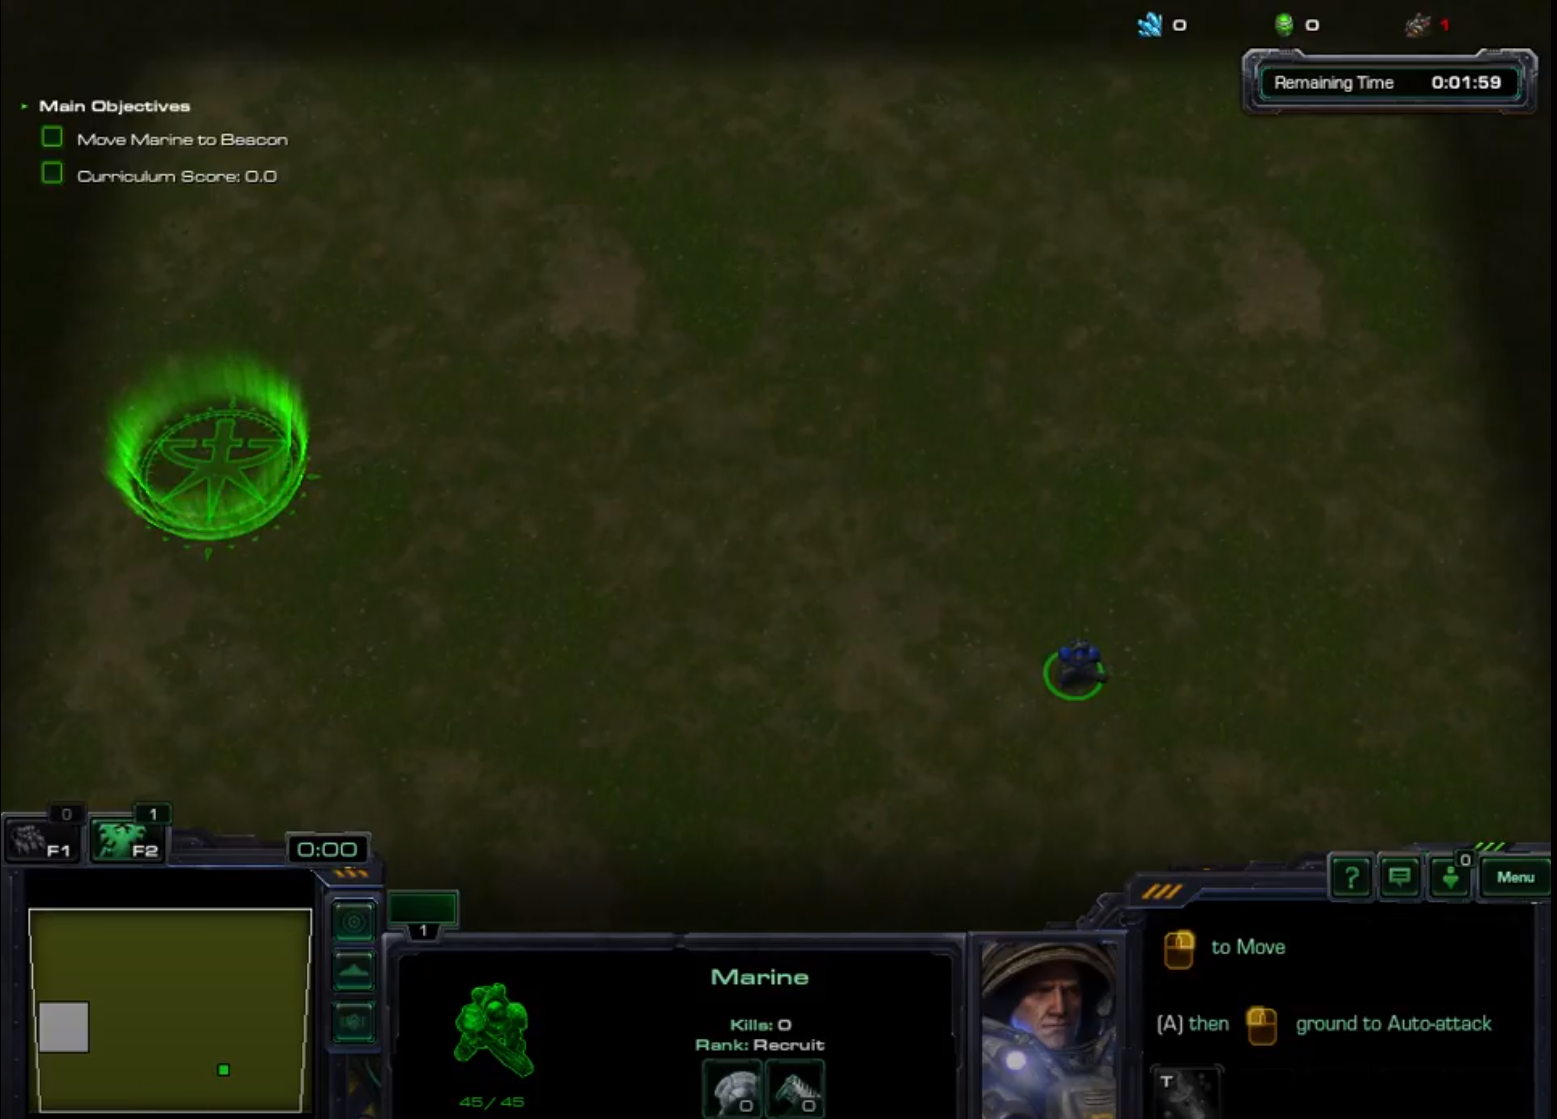
\includegraphics[width=4cm, height=3cm]{source/images/sc2_minigame_beacon_1} }
	\qquad
	\subfloat[Second Beacon]{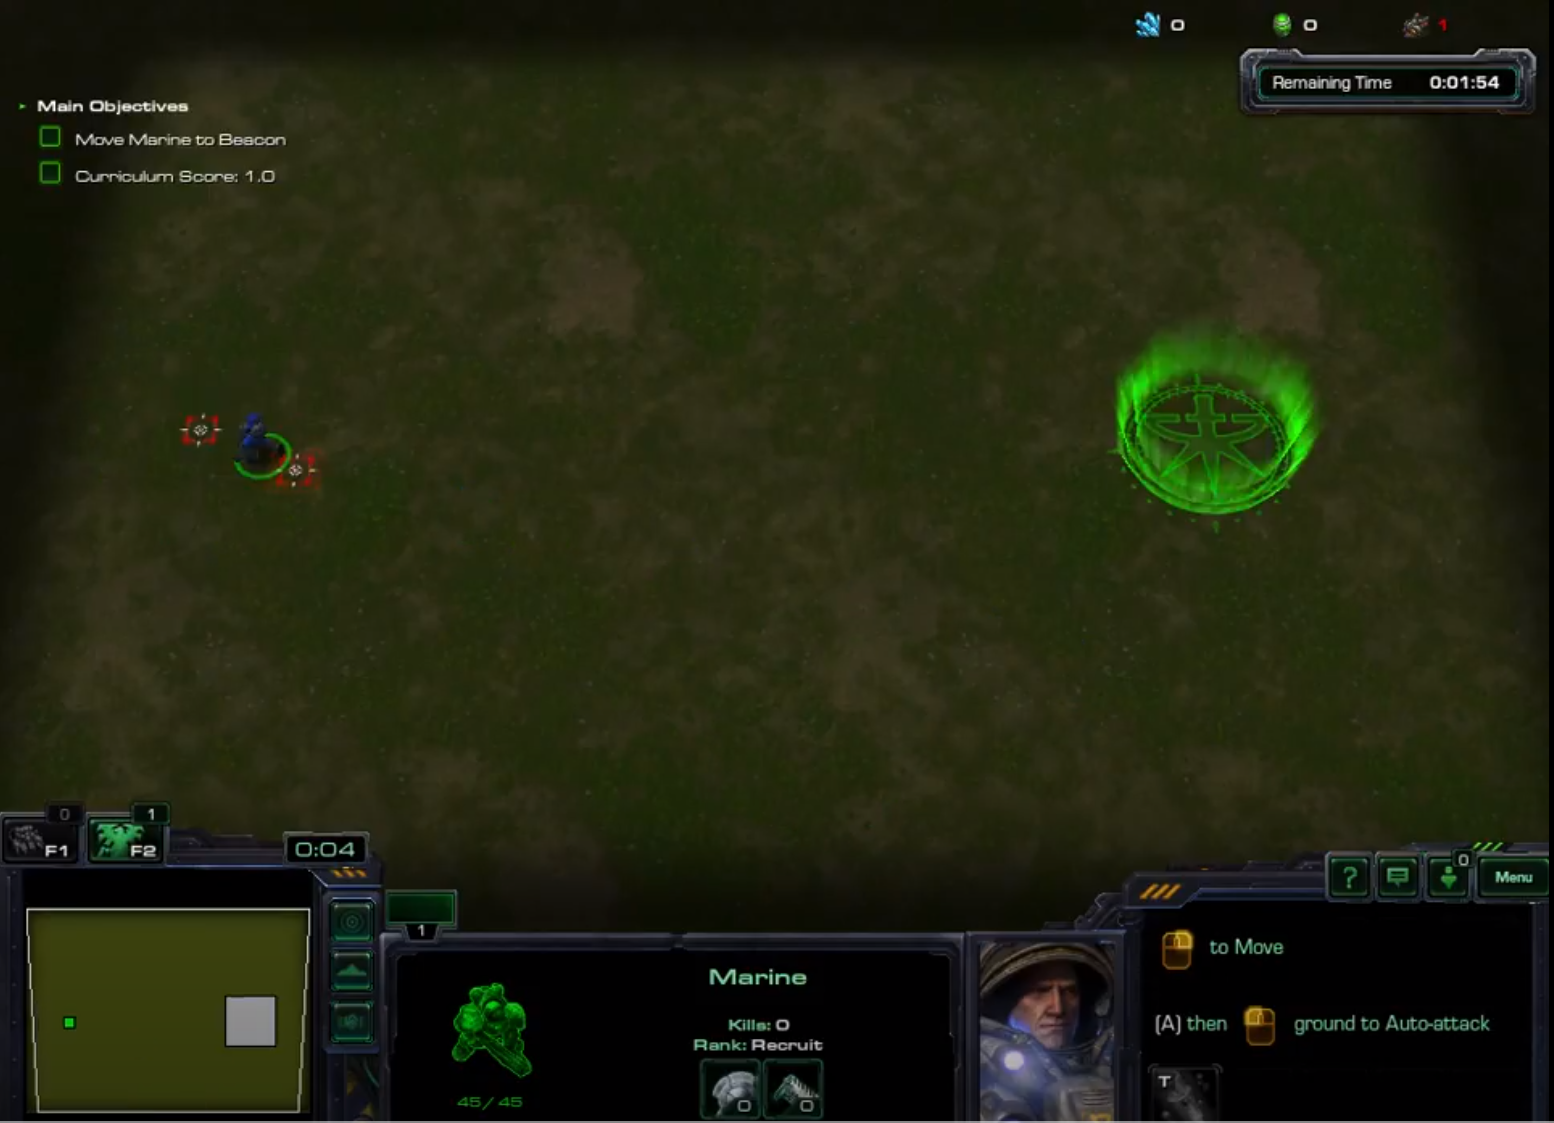
\includegraphics[width=4cm, height=3cm]{source/images/sc2_minigame_beacon_2} }
	\caption[MoveToBeacon]{MoveToBeacon. The small blue object is a unit \textit{Marine} and the green circle is the beacon. (a) is the initial state, (b) is the state after reaching the beacon. Source: Adapted from \protect\cite{sc2_beacon} }
\end{figure}
\subparagraph{CollectMineralShards}
In the mini-game CollectMineralShards the focus is the collection of minerals. Two units have to collect 20 minerals together, before new minerals spawn, repeatedly. The time limit for this mini-game is also 120 seconds and for each collected mineral a reward of +1 is given \cite{2017arXiv170804782V}.
\begin{figure}[H]
	\centering
	\subfloat[Initial state]{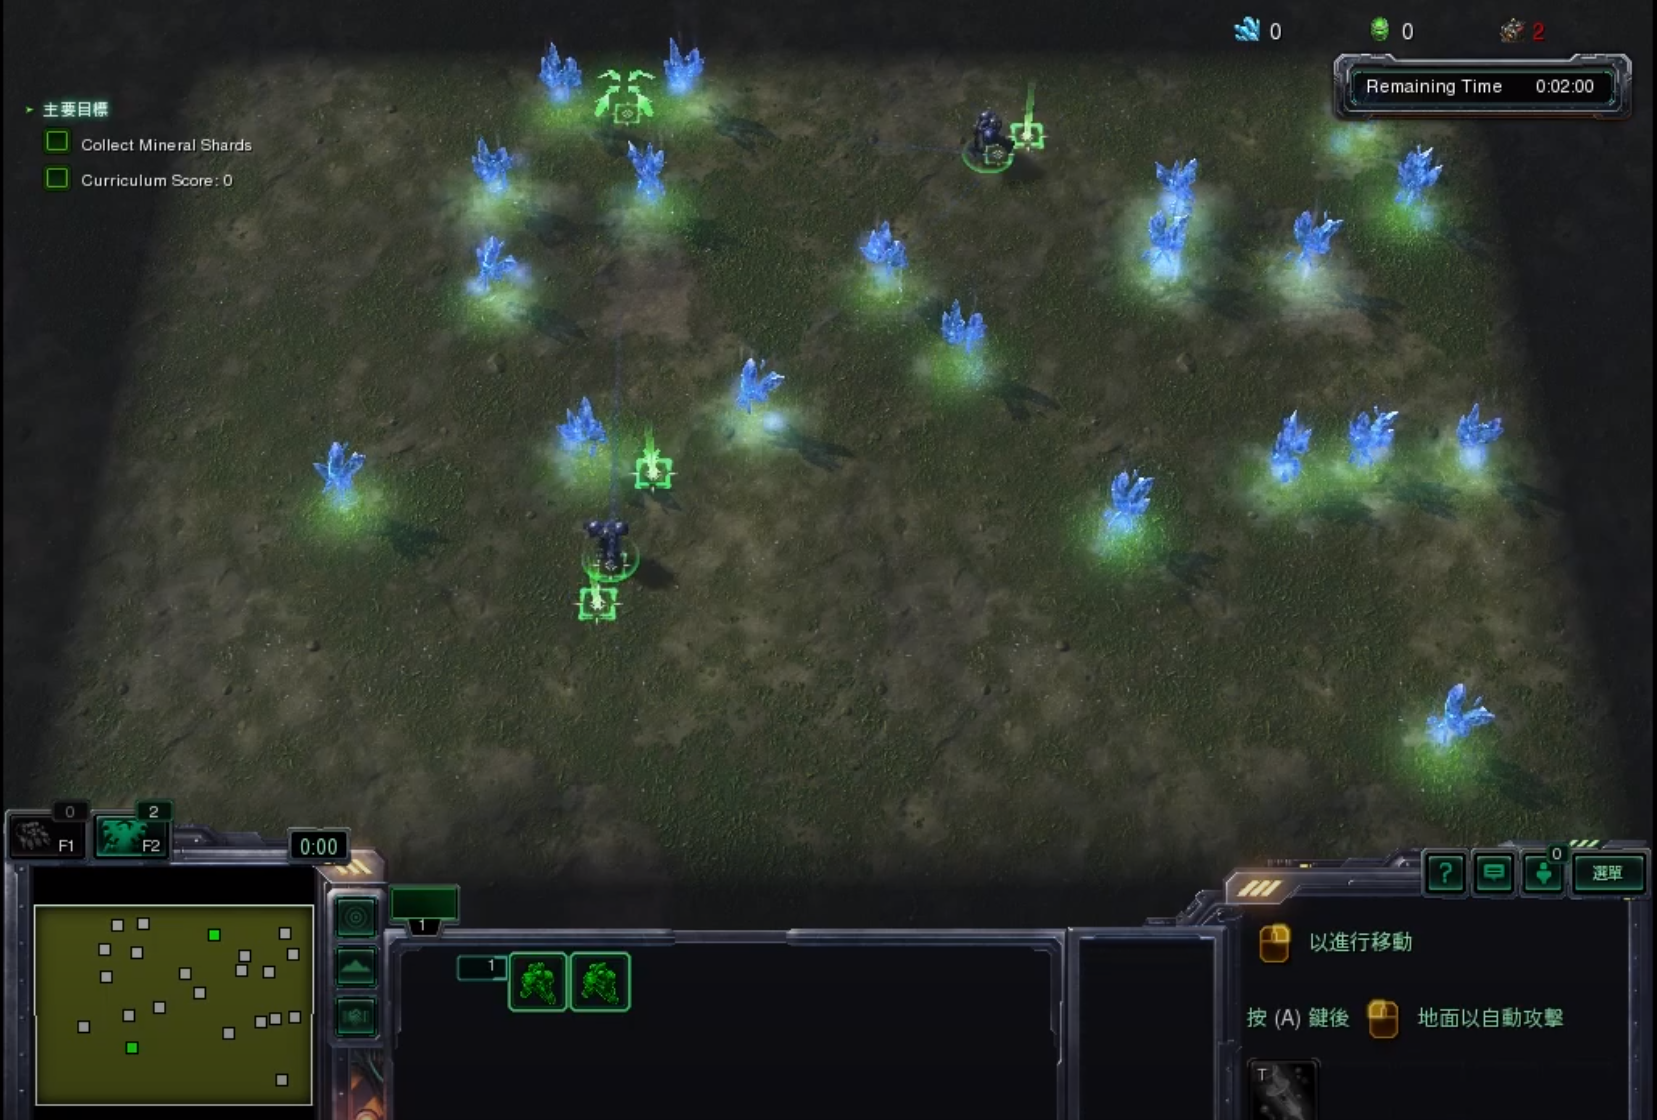
\includegraphics[width=4cm, height=4cm]{source/images/sc2_minigame_minerals_1} }
	\qquad
	\subfloat[After collecting 18 minerals]{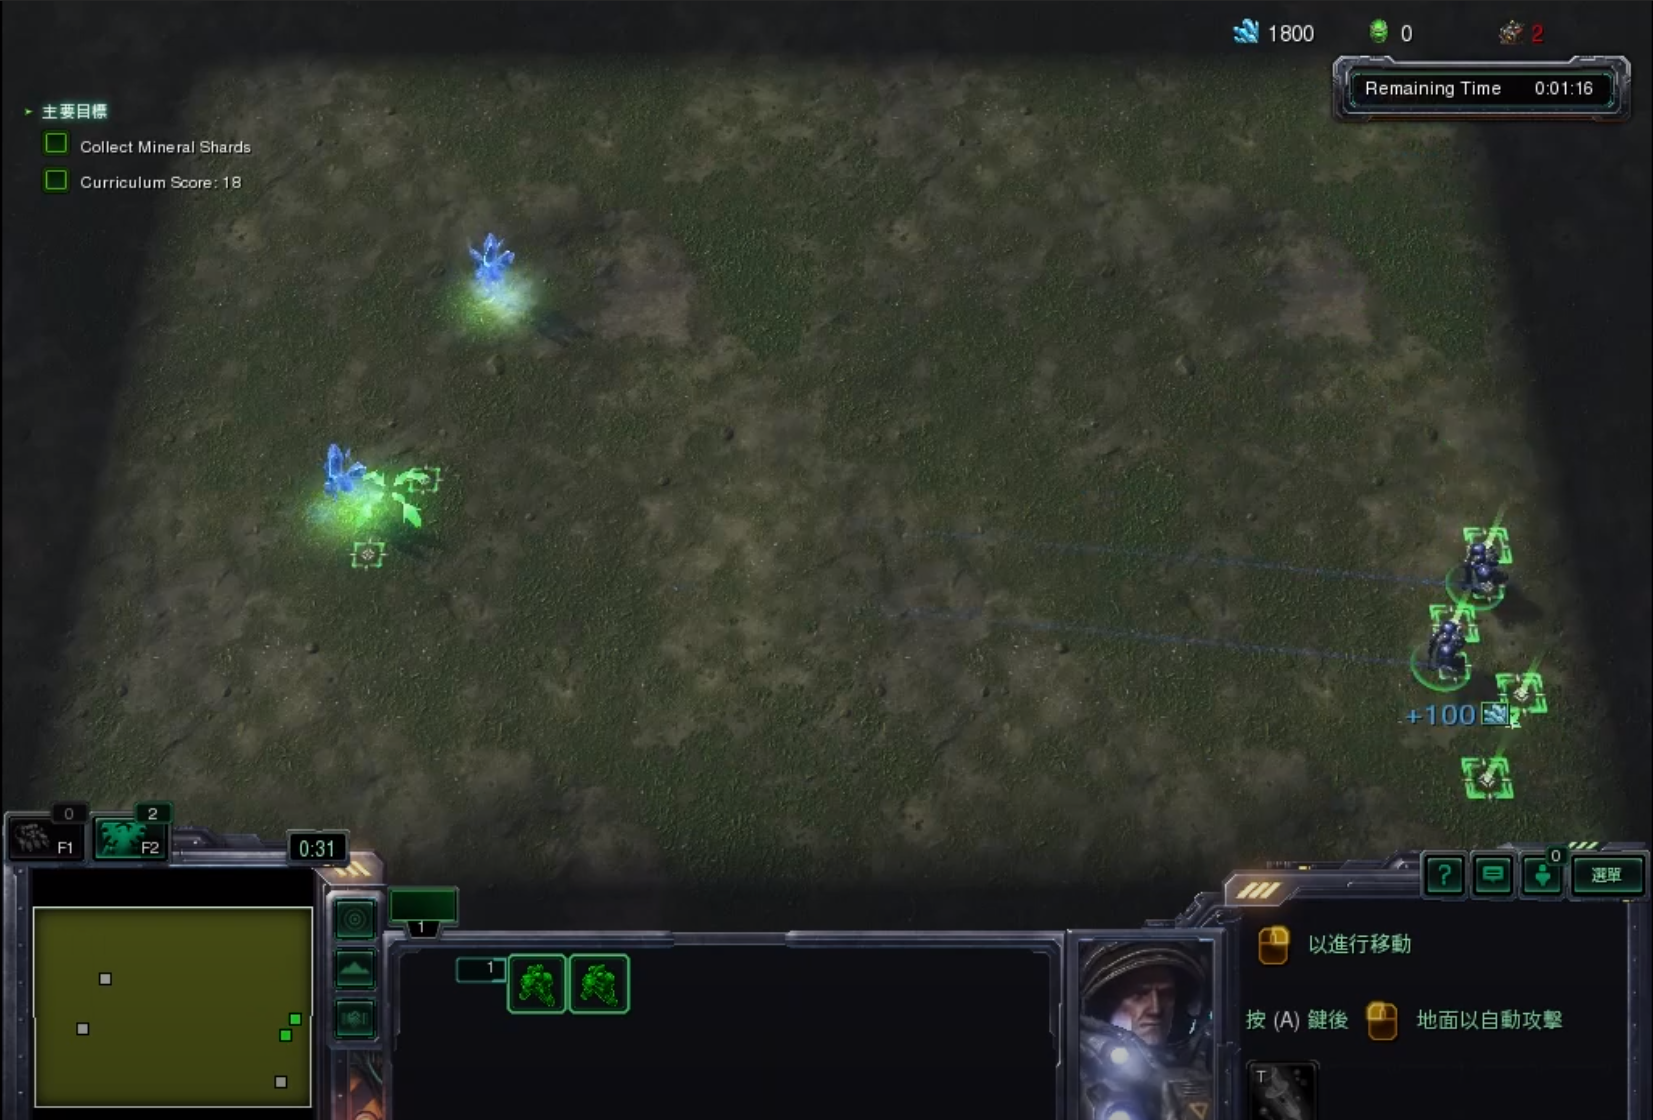
\includegraphics[width=4cm, height=4cm]{source/images/sc2_minigame_minerals_2} }
	\caption[CollectMineralShards]{CollectMineralShards. The blue crystals are the minerals. (a) is the initial state, (b) is the state after collecting 18 minerals. Source: Adapted from \protect\cite{sc2_minerals}}
\end{figure}
\subparagraph{FindAndDefeatZerglings}
For FindAndDefeatZerglings the agent has to find enemy units and destroy them. The agent has 180 seconds to defeat repeatedly 25 enemy units with three allied units. This mini-agent is more complex than the previous ones, because in the previous mini-games, the agents played with Fog of War disabled and also no camera movements were required, since the mini-games were in single-screens. Now, out of the 25 enemy units, two spawn within the vision range of the allied units and the remaining 23 units are scattered outside the vision range, in Fog of War. The rewards are also different for this mini-game, for each defeated enemy unit, the reward is +1 and when an allied unit dies, the reward is -1. Additionally, when all allied units are dead, the game is over \cite{2017arXiv170804782V}.
\begin{figure}[H]
	\centering
	\subfloat[Initial state]{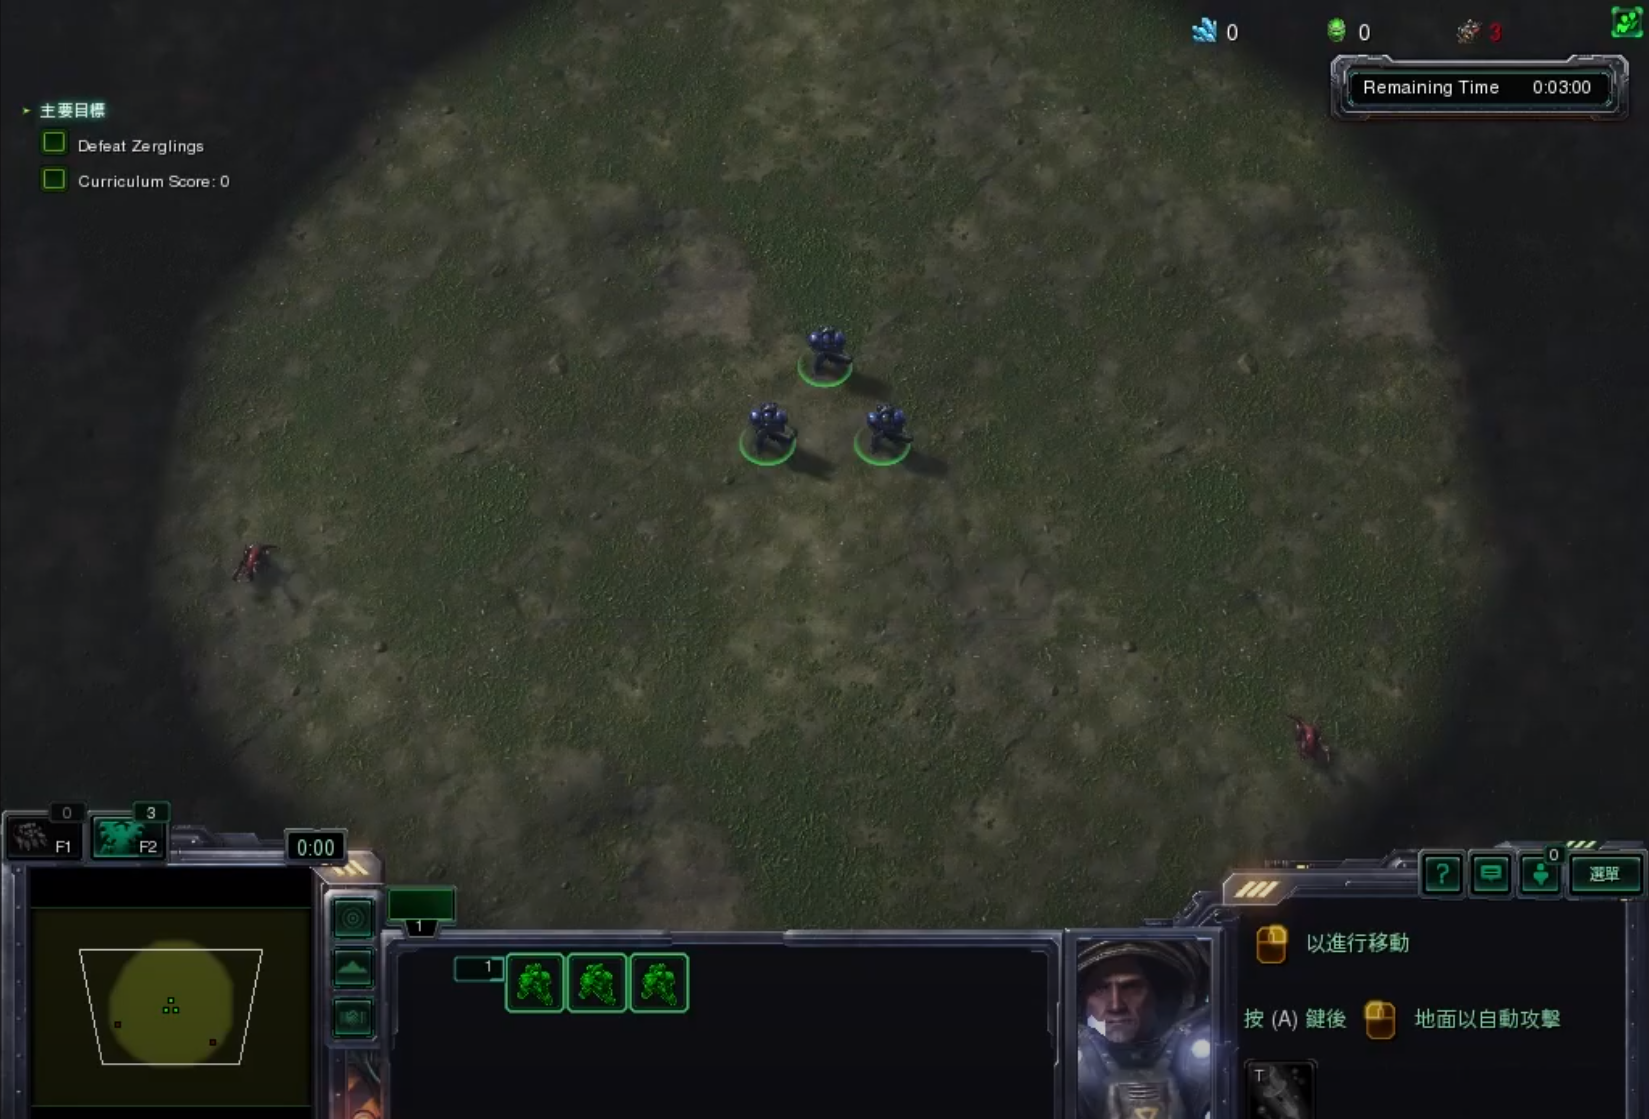
\includegraphics[width=4cm, height=4cm]{source/images/sc2_minigame_zergling_1} }
	\qquad
	\subfloat[After defeating 16 zerlings]{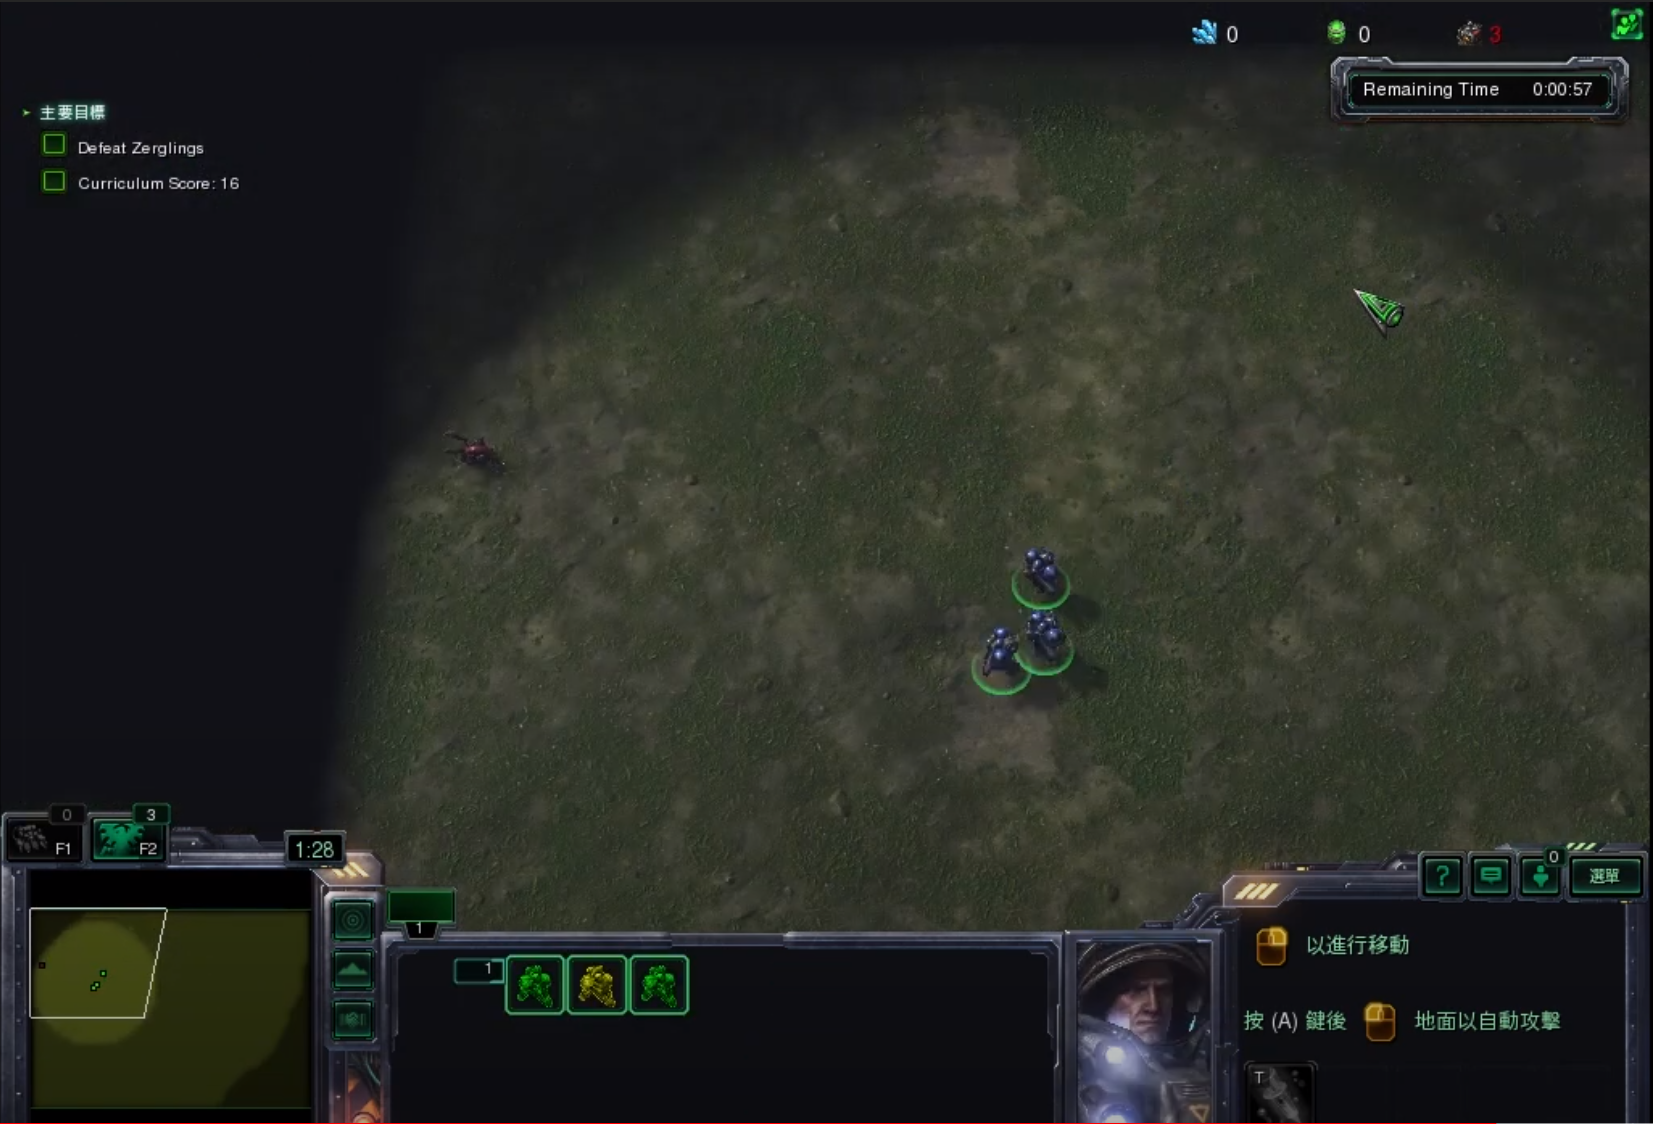
\includegraphics[width=4cm, height=4cm]{source/images/sc2_minigame_zergling_2} }
	\caption[FindAndDefeatZerglings]{FindAndDefeatZerglings. The small red creatures are the zerglings. (a) is the initial state, (b) is the state after defeating 16 zerglings. Source: Adapted from \protect\cite{sc2_zergling}}
\end{figure}
\subparagraph{Remaining Mini-Games}
The other mini-games behave similar. They have specific tasks with initial states, rewards based on actions, conditions to terminate the game and further additional settings, e.g. Fog of War, vision range \cite{2017arXiv170804782V}.

\subsection{AlphaStar} \label{ssec:alphastar}
AlphaStar is an AI developed by DeepMind that plays SC2. It is the first AI to defeat professional players and playing the game at a Grandmaster level under professional circumstances \cite{Vinyals2019}. The AI was able to do so by learning the game by different learning techniques, starting with supervised learning on replays. This technique allowed the agent to ``watch'' human replays, imitate their actions and learn essential micro and macro-strategies. The supervised agent was able to be rated in the top 16\% of human players, the Diamond rank. This agent was used as a baseline for further enhancement by RL and an algorithm for multi-agent RL. The focus of the RL algorithm was, maximizing the win rate against a variety of enemies. Agents were competing against each other in the multi-agent RL algorithm. They were split into two groups, main and exploiter agents. The main agents' focus was to win against everyone and the exploiter agents focused on helping the main agents to expose their flaws and weaknesses in order to make them stronger \cite{Vinyals2019}. 

With these techniques, AlphaStar managed to get rated within the 0.5\% of human players and by using multi-agent RL to top 0.15\%, with all three races being on Grandmaster level \cite{Vinyals2019}.

\begin{figure}[H]%
	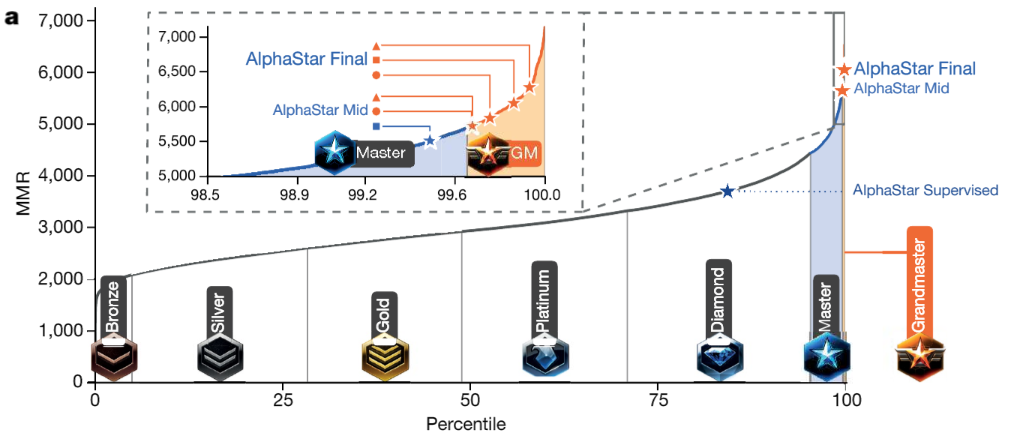
\includegraphics[width=\columnwidth]{source/images/sc2_rating}%
	\caption[SC2 Agents rating]{Agents rating. The geometric shapes refer to the different races. Triangle: Terran, Square: Protoss and Circle: Zerg. Source: Reprinted from \protect\cite{Vinyals2019}}%
	\label{fig:elo}%
	\medskip
	\small
\end{figure}

\subsection{Metrics}
DeepMind and Blizzard made different approaches to measure the performance of their agents or players which can be summarized as:
\begin{itemize}
	\item splitting a complex task into several sub-tasks, so that each task can be evaluated individually \cite{alphastarblog}
	\item using a rating system, that reflects the players skill level by accumulating points, that changes depending on victory or defeat
	\item compute APM (Action Per Minute), the total amount of actions a player performs per minute, and compare to other players  \cite{Vinyals2019}
	\item competing against pro players \cite{2017arXiv170804782V}
\end{itemize}